\section*{Quick Start Guide}

\subsection*{Kühling\&Kühling HT500.3}

 Congratulation, you seemingly just received your HT500.3 3D Printer. Read the following instructions thoroughly and you are up and running in no time.

You will always find the latest version of the manual, additional documentation and new software releases at

http://docs.kuehlingkuehling.de

Please visit our site regularly so that you do not miss important developments and new features. 


\subsection*{Components overview}

\begin{figure}[H]
  \centering
  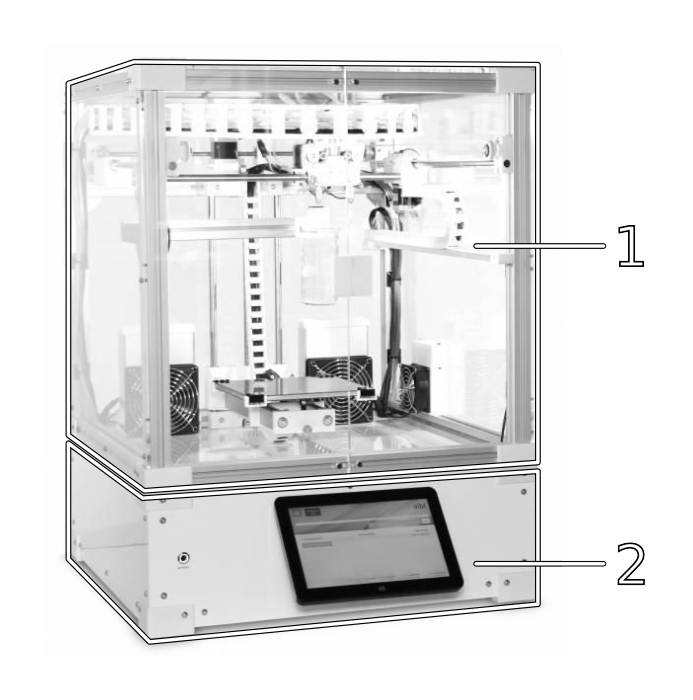
\includegraphics[width=.7\linewidth]{./img/qsg_overview_1.png}
  \caption{The two main functional sections of the HT500 3D Printer: the build 
           chamber with the functional components and the electronic chamber containing the regulation electronics.}
\end{figure}

\begin{table}[H]
  \centering
  \begin{tabulary}{\textwidth}{ L L }
    \toprule
    No. &   Description         \\
    \midrule
    1 	&   Build chamber       \\
    2 	&   Electronic chamber  \\
    \bottomrule
  \end{tabulary}
\end{table}

\begin{figure}[H]
  \centering
  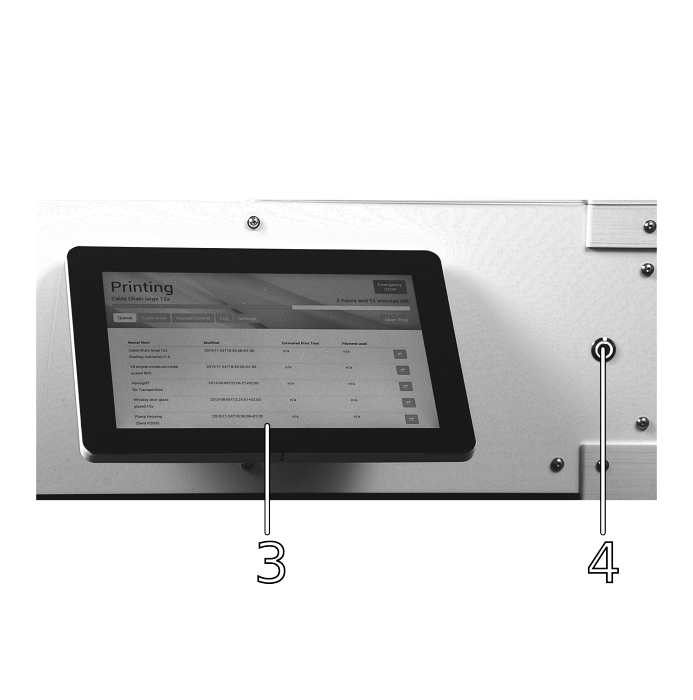
\includegraphics[width=.7\linewidth]{./img/qsg_overview_2.png}
  \caption{HMI touchscreen for direct operation and wake button at the front panel.}
\end{figure}


\begin{table}[H]
  \centering
  \begin{tabulary}{\textwidth}{ L L }
    \toprule
    No. 	&   Description  \\
    \midrule
    3 	    &   Operating screen \\
    4 	    &   Wake button  \\
    \bottomrule
  \end{tabulary}
\end{table}


\begin{figure}[H]
  \centering
  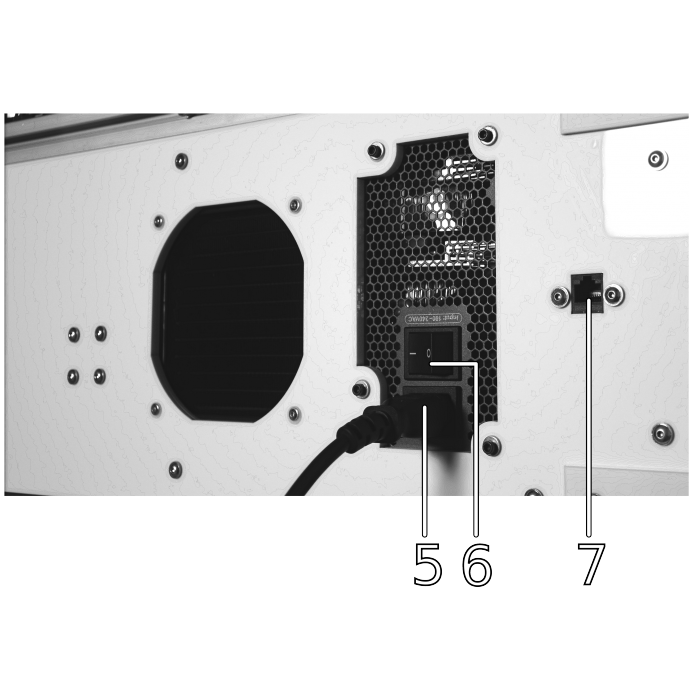
\includegraphics[width=.7\linewidth]{./img/qsg_overview_3.png}
  \caption{Power/network connections and mains switch at the rear panel}
\end{figure}

\begin{table}[H]
  \centering
  \begin{tabulary}{\textwidth}{ L L }
    \toprule
    No. 	&   Description  \\
    \midrule
    5 	    &   Mains socket  \\
    6 	    &   Main switch   \\
    7 	    &   RJ45 ethernet socket   \\
    \bottomrule
  \end{tabulary}
\end{table}


\begin{figure}[H]
  \centering
  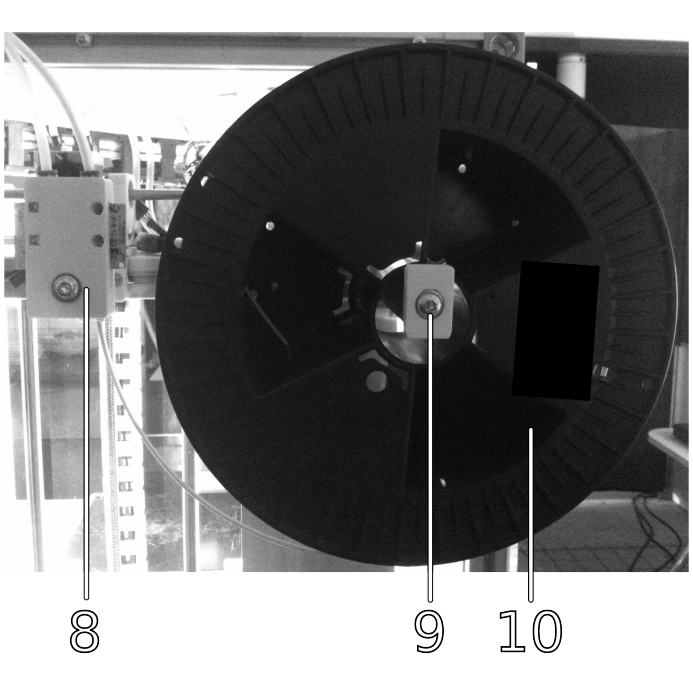
\includegraphics[width=.7\linewidth]{./img/qsg_overview_4.png}
  \caption{Filament feed system at the rear of the build chamber}
\end{figure}


\begin{table}[H]
  \centering
  \begin{tabulary}{\textwidth}{ L L }
    \toprule
    No. 	&   Description  \\
    \midrule
    8 		&   Filament inlet with limit switches  \\
    9 		&   Filament spool carrier  \\
   10 		&   Filament spool   \\
    \bottomrule
  \end{tabulary}
\end{table}


\subsection*{Safety precautions}

\begin{danger}
  ELECTRICAL HAZARD
  All electrical equipment inside the 3D Printer has been designed and built in accordance with the regulations stated in the Low Voltage Directive 2006/95/EG (see Declaration of Conformity) and established electrical engineering practice with all necessary respect to the user's safety.
  Regard that handling electrical equipment always implies risks that require special care.
  To avoid electrical shock and burning injuries and damage to the 3D Printer:
  \begin{itemize}  	
    \item Only connect the 3D Printer to the specified supply voltage.
    \item Do not operate the 3D Printer with defective cable connections.
    \item Do not set up the 3D Printer in a moist environment.
  \end{itemize}
\end{danger}

\begin{danger}
  OF CUTTING INJURIES AND EYE DAMAGE
  The packing straps are pretensioned and may whip when cut, causing cutting injuries or eye damage. 
  \begin{itemize} 
  	\item Hold down the top part of the strap and cut it at the side. 
  	      Make sure it does not hit somebodies face.  
  \end{itemize}
\end{danger}

\begin{danger}
  The 3D Printer weighs 50kg (empty). Dropping or toppling of the 3D Printer may cause crushing injuries. Lifting the printer on yourself can cause back injuries. 
  \begin{itemize} 
  	\item Always carry the 3D Printer \emph{two by two} and hold it from beneath the 
  	      bottom edges.
  \end{itemize}
\end{danger}

\begin{danger}
  The transport box is made of unfinished plywood and may hold splinters and sharp edges that can cause cutting injuries. 
  \begin{itemize} 
  	\item Take care when removing the transport packaging and wear protective 
  	      gloves. 
  \end{itemize}
\end{danger}

\begin{notice}
  If the 3D Printer has a temperature below 16\degree C (e.g. directly after delivery in cold weather) there is a danger of air humidity condensing on sensitive electronic components. This can lead to severe damages due to short circuiting during commissioning.
  Therefore, it is necessary to thoroughly let the 3D Printer warm up to ambient temperature for at least 12 hrs. at its operating place prior to commissioning.
  Regard the \emph{ambient conditions} required for operation. 
\end{notice}

\begin{notice}
  In order to ensure your own safety and the proper functioning of your HT500.3 during operation read and observe the safety instructions in the online documentation. 
\end{notice}


\subsection*{Installation requirements}

\begin{itemize}
  \item For optimal operation a free space according to the adjacent picture should 
        be provided.
  \item The substructure of the 3D Printer must be stable and weight carrying with a 
        minimum payload of 60kg and a flat surface.
  \item No tablecloth must be placed underneath the 3D Printer to avoid blocking the 
        ventilation openings in the bottom. Loss of air flow can lead to severe damage by overheating of the drives.
  \item The 3D Printer \emph{must not} be set up in a surrounding with high 
        formation of dust (e.g. near woodworks, grinding workplaces etc.). Ingress of particles into the filament feed system can lead to intense cleaning efforts due to clogging of the nozzle tips and thus immense non-productive time.
  \item Also ensure that the 3D Printer cannot topple, slide or tilt due to 
        operating vibrations.
  \item A 110 - 230 V(AC) power source must be within reach of the power cable (1 m).
  \item Your network must provide DHCP IP address management and should be connected 
        to the internet to enable the 3D Printer to fetch current time signal via Network Time Protocol (ntp).
        Refer to the online manual if your network is built differently.
\end{itemize}

\begin{figure}[H]
  \centering
  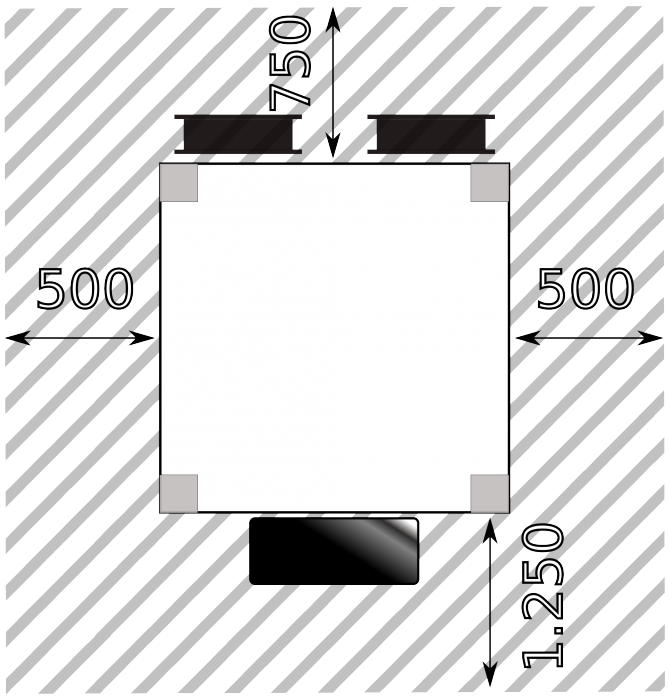
\includegraphics[width=.7\linewidth]{./img/qsg_workspace.png}
  \caption{Free space required for optimal operation of the HT500.3 3D Printer.}
\end{figure}


\subsection*{Setup}

\begin{itemize}
  \item Cut and remove the packing straps around the transport box.
  \item Open the wooden transport box's lid and lift the plywood frame off the 
        pallet in one piece.
  \item Cut and remove the packing straps around the 3D Printer.
  \item Remove the wooden panel and foam wrap on top of the 3D Printer.
  \item Take out the accessory kit box.
  \item Lift the 3D Printer onto the prepared pedestal.
  \item Remove all transport securing devices (blue tape and the cardboard 
        underneath the print bed).
  \item heck the entire device carefully for any transportation damage and 
        completeness of delivery.
\end{itemize}


\subsection*{Connecting, turning on and accessing the 3D Printer}

\begin{itemize}
  \item Plug the mains cable into the mains socket at the rear cover and connect the 
        3D Printer to the power supply.
  \item Connect the 3D Printer to the local network via the RJ45 plug at the rear 
        cover.
  \item Toggle the main switch at the rear cover to <I> (ON).
  \item It may take a few minutes until the touchscreen has fully loaded the 
        operating screen - wait patiently without interfering. The first screen will be the \emph{Print} screen with the (empty) print-job queue and the top-left status message displaying {Idle}.

    \begin{figure}[H]
      \centering
      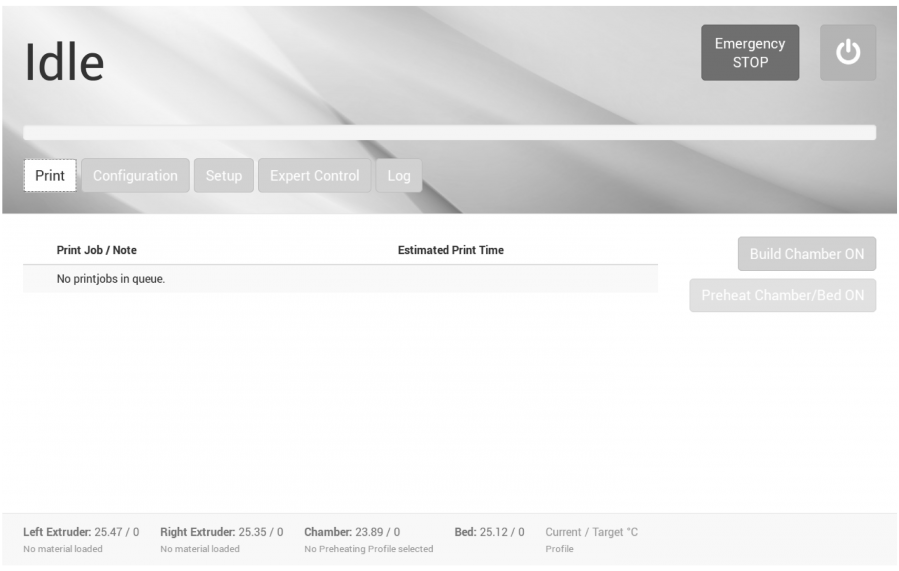
\includegraphics[width=.7\linewidth]{./img/qsg_emptyprintscreen.png}
      \caption{After the boot sequence the operating screen starts with the PRINT 
               tab in IDLE mode. At initial commissioning, the print-job queue is empty and no temperature profiles are selected.}
    \end{figure}
  
  \item Switch to the \emph{Setup} tab via the respective button in the header.
  \item Write down the \emph{Web Interface URL} displayed on the right half of the 
        screen.

    \begin{figure}[H]
      \centering
      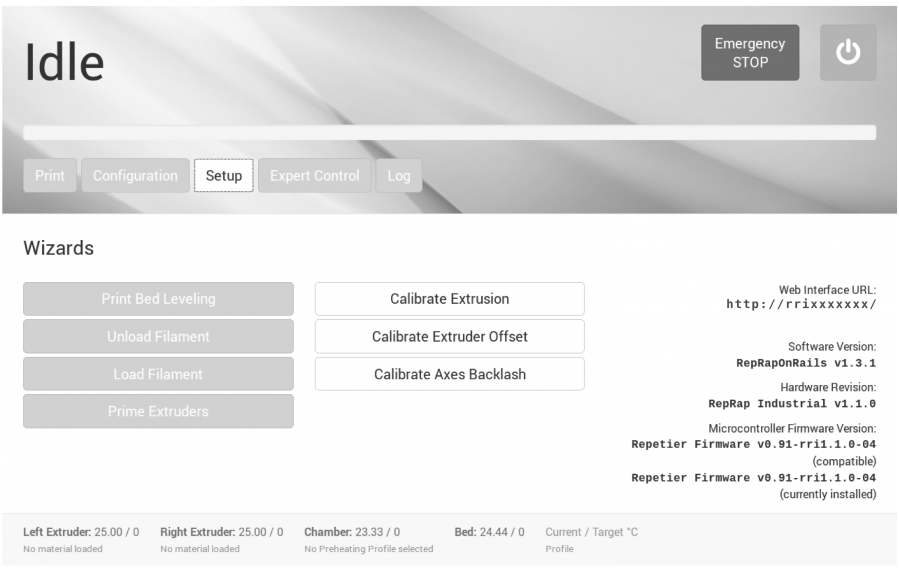
\includegraphics[width=.7\linewidth]{./img/qsg_setupurl_fullscreen.png}
      \caption{The Web Interface URL on the SETUP screen is required for connecting 
               the 3D Printer with your local network.}
    \end{figure}

  \item Now open your web browser on your PC and enter the web interface URL in the 
        address line and you will be greeted with the \emph{First Steps} screen that provides a direct link to the online manual.

    \begin{figure}[H]
      \centering
      
\includegraphics[width=.7\linewidth]{./img/qsg_wif_firststeps.png}
    \end{figure}

\end{itemize}

All further steps are explained in in the Initial Commissioning section of the user's manual available 
under \verb|https://docs.kuehlingkuehling.de/|

That's it - your HT500.3 3D Printer is ready for the first print.
Proceed with the instructions provided in the user's manual to perform your first prints and familiarize with your 3D Printer.

